\chapter{Trigger Logic and Data Taking}
\label{sec:trigger}
The trigger system that we need is a logic circuit that will be able to select muons
that do not cross the setup. Thus, we can retrieve a signal of a stopping muon 
that can be used as a start signal 
for the time measurement of the decay.
If we take \autoref{fig:Setup} as reference of the experimental apparatus 
each of the half-planes of plane 0 have two PMTs, which will be connected with an AND gate.
The two half-planes with an OR gate in this way only the signal
that activate the two PMTs can enter the circuit as can be seen in \autoref{fig:logig_plane0}.
By doing this, we avoid detecting to much background.
Meanwhile the OR gate is needed since there are two half-planes
and a muon can cross either two.\\
\begin{figure}[h]
\begin{center}
\includegraphics[width=80 mm,scale=0.5]{figures/Cattura2.png}
\end{center}
\caption{Logic circuit of plane 0.}
\label{fig:logig_plane0}
\end{figure}
We repeat the process for plane 1. For plane 2
we want a NOT gate at the end of the OR gate, so that we have a signal when no muons cross P2
to make sure that the muon has actually stopped. The P0, P1 and NOT P2 will be connect to an AND
gate so that only when all of them generate a signal we can have the Trigger signal as
shown in \autoref{fig:trigger_system}.

\begin{figure}[h]
\begin{center}
\includegraphics[width=100mm]{figures/Cattura3.png}
\end{center}
\caption{Trigger system.}
\label{fig:trigger_system}
\end{figure}

For the time measurement we use a couple of TDCs in series since we need a least 10$\;\symup{\mu}$s
and the max time measurable for this TDC is 5$\;\symup{\mu}$s.
The TDC is controlled by a crate controller that sends the information 
from the module. The crate controller works with a DAQ code (labview) 
that creates memory location that will be read by the crate which will give command to the
CAMAC module in this way
\begin{enumerate}
  \item if and only 1 of the clock of the TDC has a stop before the time limit (5$\;\symup{\mu}$s) then a memory location called LAM is set to 1
  \item  the create read continusly the memory location of the LAM, if it's 1 the create controller stop the reading the LAM read the measurement and then clear them to start again
\end{enumerate}
 The problem is that if there are no stopping signal the LAM wil never be set to 1 and we
  have a DAQ hanging problem. The solution is given by taking a copy of the start signal
dealy it by 4.7$\;\symup{\mu}$s and connect it to one of the clock in this way we have
a fake stop to prevent the problem. With this in mind we build the circuit shown in \autoref{fig:daq}.\\
\begin{figure}[h]
\begin{center}
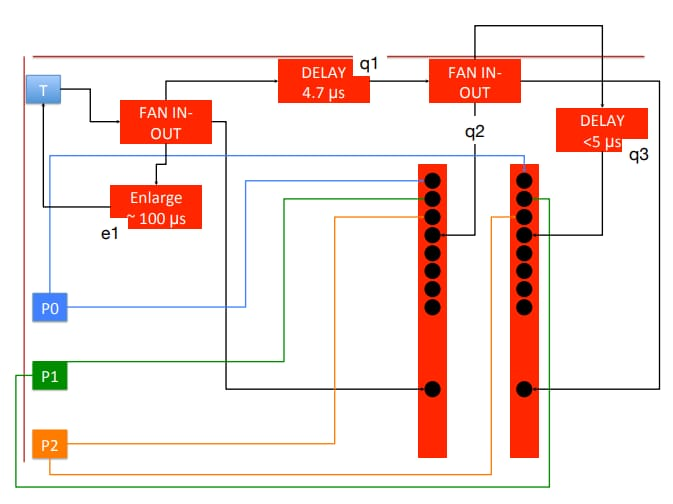
\includegraphics[width=100mm]{figures/cattura4.png}
\end{center}
\caption{Data aquistion circuit.}
\label{fig:daq}
\end{figure}

The first three clocks will be connected to the P0, P1 and P2 in search for an electron
apparence signal. The start for the first TDC in given by the trigger and then we take a copy
of it and delay it by 4.7$\;\symup{\mu}$s (q1). From this we take 3 copy with a fan-in-fan-out :
\begin{enumerate}
\item the first will be used as the fake stop for the first TDC (q2)
\item the second will be the start of the second TDC
\item the third will be delayed again by a time $<5\;\symup{\mu}$s and used as a fake stop for the second TDC (q3)
\end{enumerate}
The last thing is to make sure that no trigger is genereted in the deadtime of the DAQ
so we take the signal enlarge it up to 100$\;\symup{\mu}$s and send back to the logic
unit that provide the trigger in the VETO input (e1).\\
